\section{Task 6 --- Initial Vector (IV) and Common Mistakes}
%
\subsection{IV Experiment}
%

\begin{figure}
    \centering
    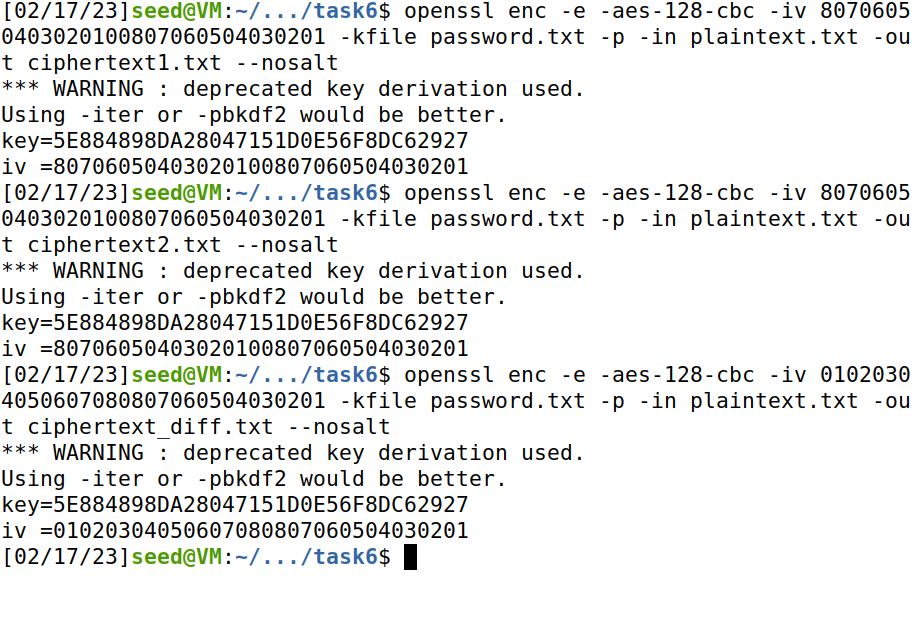
\includegraphics[height=\textheight,width=\textwidth,keepaspectratio]
    {figures/generate_cipher_dif_IV.png}
    \caption{OpenSSL commands to generate ciphertexts.}\label{fig:diff_IV_script}
\end{figure}

\begin{figure}
    \centering
    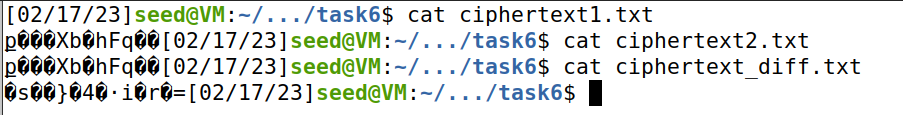
\includegraphics[height=\textheight,width=\textwidth,keepaspectratio]
    {figures/result_diff_IV.png}
    \caption{Resulted ciphertexts with the same and different IVs.}\label{fig:ciphertext_IV}
\end{figure}

In this experiment, we stored ``Hello World!'' in the {\fontfamily{qcr}\selectfont plaintext.txt}
file. Then we would encrypt it with the same IV and key, resulting in {\fontfamily{qcr}\selectfont
ciphertext1.txt} and {\fontfamily{qcr}\selectfont ciphertext2.txt}. In the second case, we
encrypted {\fontfamily{qcr}\selectfont plaintext.txt} using the same key but with a different
IV from the first case.

We used IV1 {\fontfamily{qcr}\selectfont 80706050403020100807060504030201} for files
{\fontfamily{qcr}\selectfont ciphertext1.txt and ciphertext2.txt}; 
IV2 {\fontfamily{qcr}\selectfont 01020304050607080807060504030201} for
{\fontfamily{qcr}\selectfont ciphertext\_diff.txt} file.

As you can see in \autoref{fig:ciphertext_IV}, identical IV and key generates the same
ciphertext. In contrast, even you encrypt with the same key but a different IV, it
will produce a different ciphertext.

\subsection{Common Mistake: Use the Same IV}
%
\begin{lstlisting}[language=python, caption=A script that finds
    the orginal text P2 (OFB mode).]
#!/usr/bin/python3

# XOR two bytearrays
def xor(first, second):
   return bytearray(x^y for x,y in zip(first, second))

P1   = "This is a known message!"
C1 = "a469b1c502c1cab966965e50425438e1bb1b5f9037a4c159"
C2 = "bf73bcd3509299d566c35b5d450337e1bb175f903fafc159"

# Convert ascii string to bytearray
P1_byte = bytes(P1, 'utf-8')

# Convert hex string to bytearray
C1_byte = bytearray.fromhex(C1)
C2_byte = bytearray.fromhex(C2)

o1 = xor(P1_byte, C1_byte) # output of encryption block | P1 XOR C1
P2_byte = xor(C2_byte, o1) # plaintext of the ciphertext C2 | O1 XOR C2

print(str(P2_byte, 'utf-8'))
\end{lstlisting}

\begin{figure}
    \centering
    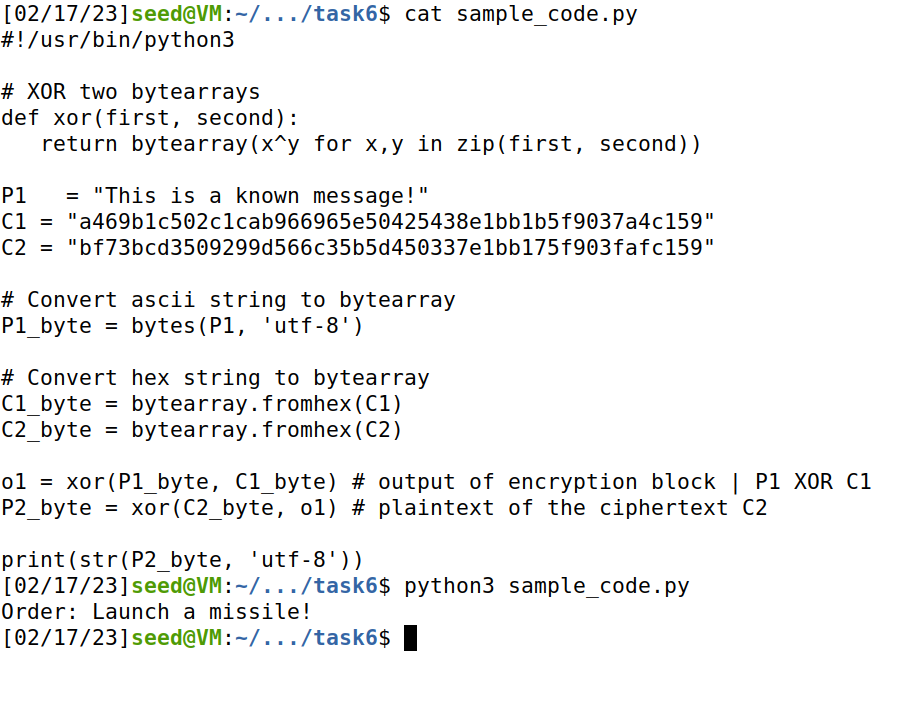
\includegraphics[height=\textheight,width=\textwidth,keepaspectratio]
    {figures/same_IV_OFB.png}
    \caption{Plaintext P2 generated by the Python script.}
    \label{fig:p2_script}
\end{figure}

In the OFB mode (see \autoref{fig:ofb_dec}), the key for the second block is an output
of \(E_{1} = Enc(IV,Key)\). And the key for the \(i^{th}\) block is \(E_{i}
= Enc(E_{i-1},Key)\). Hence, if the same IV and Key are used, the subsequent keys
for following blocks are identical, generating identical \(E_{i}\). Taking advantage of
this point, firstly we XORed a pair of ciphertext and plaintext, \(C1 and P1\) in this
case, which generates the \(E_1\). As same IV and Key are used, \(E_i\) is identical at
all blocks. Hence, a plaintext \(P2\) can be reproduced by \(P2 = E_i \oplus C2\).

The plaintext \(P2\): {\fontfamily{qcr}\selectfont Order: Launch a missile!}

In the CFB mode (see \autoref{fig:cfb_dec}), only the first block can be reproduced as
the same way in OFB mode, which is decribed above. Since a ciphertext is fed into the
encryption scheme of the next block \(E_i = Enc(C_{i-1},Key)\), different \(E_i\)
at all blocks under different ciphertext block. Hence, even same IV and Key are used,
we can only reproduce the first block.

\subsection{Common Mistake: Use a Predictable IV}
%
Look at \autoref{fig:cbc_mode}, Bob's first ciphertext block is generated by: \(C_{Bob}
=Enc(Key, IV_{Bob} \oplus P_{Bob})\). If Eve can know the IV values used to genereate
\(C_{Bob}\) and the next ciphertext and the limited instances of Bob's secrets
, ``Yes'' or ``No'' in this case, he can do a chosen-plaintext attack. Guessed
plaintext by Eve is \(P_{guessed-Eve}\). The mathematical formula for CBC encryption
of the first blockl is:
\begin{math}
    C_{Eve} = Enc(Key, IV_{Eve} \oplus P_{Eve})
\end{math}

If Eve tricks the plaintext such that \(P_{Eve} = P_{guessed-Eve} \oplus IV_{Eve}
\oplus IV_{Bob}\), then the output ciphertext becomes:
\begin{math}
    C_{Eve} = Enc(Key, IV_{Eve} \oplus P_{guessed-Eve} \oplus IV_{Eve}
    \oplus IV_{Bob})\\
    C_{Eve} = Enc(Key, P_{guessed-Eve} \oplus IV_{Bob})
\end{math}

So if \(C_{Eve}=C_{Bob} \Rightarrow P_{Bob}=P_{guessed-Eve}\), Eve guesses Bob's
secret correctly.

Back to this task, we firstly guessed that ``Yes'' is Bob's secret (see
\autoref{fig:chosen_plaintext_attack}):

\begin{itemize}
    \item Chosen plaintext ``Yes'': {\fontfamily{qcr}\selectfont 5965730d0d0d0d0d0d0d0d0d0d0d0d0d}
    \item Next IV: {\fontfamily{qcr}\selectfont ca43f358cba8d49baac2c91abf0097ac}
    \item IV used: {\fontfamily{qcr}\selectfont d56ac8e4caa8d49baac2c91abf0097ac}
\end{itemize}

We XORed three of above values and obtained:\\
{\fontfamily{qcr}\selectfont 464c48b10c0d0d0d0d0d0d0d0d0d0d0d}\\
as the plaintext need to be fed into the cipher scheme (\(P_{Eve}\)).
Then we got the output ciphertext (\(C_{Eve}\)):\\
{\fontfamily{qcr}\selectfont efdf6fe4b7f660e6abe83a781cff4f9869f04386ccba3a039828563e7b9135c6}.\\
Without the padding bytes, it matches the Bob's ciphertext:\\
{\fontfamily{qcr}\selectfont efdf6fe4b7f660e6abe83a781cff4f98}\\
(see \autoref{fig:chosen_plaintext_attack}). Hence, Bob's secret is \textbf{Yes}.

\begin{figure}
    \centering
    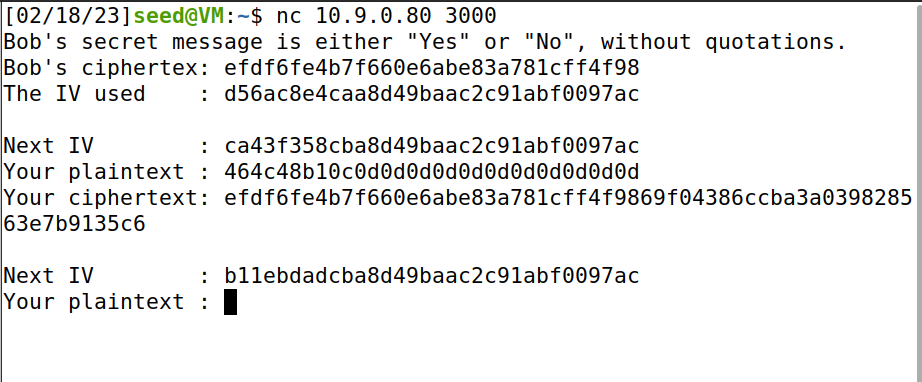
\includegraphics[height=\textheight,width=\textwidth,keepaspectratio]
    {figures/task6_yes.png}
    \caption{Chosen-plaintext attack in the CBC mode.}\label{fig:chosen_plaintext_attack}
\end{figure}